% Když budete cokoli psát: ukládejte starší verze vždy odděleně, abyste se 
% k nim mohli kdykoli vrátit. Kusy textu, které jste se rozhodli nepoužít, taky ukládejte do zvláštního souboru. Smazat se to dá vždycky, ale psát to znova je opruz. 

% A POŘÁD ZÁLOHUJTE. POŘÁD !!!

\documentclass[12pt, a4paper, oneside]{article} 
% velikost písma, stránky, typ dokumentu -- detaily viz literatura

\usepackage{czech} % nastavení češtiny
%\usepackage[latin2]{inputenc}
%\usepackage[cp1250]{inputenc} % pro win1250
\usepackage[utf8]{inputenc}
\usepackage{wrapfig} % nastavení obtékání textu
\usepackage{graphicx,amsmath} % nastavení grafiky, matematiky
\usepackage{subfig} % více obrázků vedle sebe 
\usepackage{float}

\usepackage{tocloft} %přidá tečky do obsahu ke kapitolám /sekcím 
\renewcommand{\cftsecdotsep}{\cftdotsep}

\usepackage[bookmarksopen,colorlinks,plainpages=false,linkcolor=black,urlcolor=blue,citecolor=black,filecolor=black,menucolor=black,unicode=true]{hyperref}
%bookmarksopen -- open up bookmark tree 
%colorlinks -- zbarví odkazy (implicitně orámovaný nezbarvený text)
%urlcolor -- barva odkazů (implicitně magenta) 
%linkcolor=black -- barva odkazů v obsahu (implicitně red)


% \usepackage{parskip} -- zapne americké odstavce v celé práci

\addtolength{\textwidth}{-2mm} 
\addtolength{\hoffset}{4mm}  % posun textu kvůli kroužkové vazbě  

\setlength{\intextsep}{5mm} % nastavení mezery okolo obrázků

% nastavení příkazu >\figcaption pro popis čehokoli, jako by to byly obrázky 
\makeatletter   
\newcommand\figcaption{\def\@captype{figure}\caption}
\makeatother

\def\refname{Literatura} 
% přejmenuje anglický název Reference na české Literatura


%\makeindex % příprava pro výrobu indexu (jestli ho chcete)

%%    VLNKA <fileinput>  KkSsVvZzOoUuAaIi        
% Defaultni  koncovka pro <fileinput> je  ".tex"
%FIXME: haze error
%\cstieon % Vypne chovani vlnky jako tvrde mezery v matematickem rezimu

%%%%%%%%%%%%%%%%%%%%%%%%%%%%%%%%%%%%%%%%%%%%%%%%%%%%%%%%%%%%%%%
%V PROSTŘEDÍ ROVNIC SE NESMÍ VYSKYTOVAT PRÁZDNÝ ŘÁDEK
%
%PROGRAMY VLNKA A CSINDEX SE MUSÍ SPUSTIT SAMOSTATNĚ
%%%%%%%%%%%%%%%%%%%%%%%%%%%%%%%%%%%%%%%%%%%%%%%%%%%%%%%%%%%%%%%

% definice příkazů 
\newcommand{\D}{\medskip \noindent} % nový odstavec v "americkém" formátování 
\newcommand{\B}{\textbf} %tučné písmo
\newcommand{\A}{\mathbf} %tučné písmo v matematickém režimu
\newcommand{\TO}{\ensuremath{\boldsymbol\Omega}} % tučný znak velké omega -- pro ohmy
\newcommand{\I}{\index}  % vytváří položku indexu (asi nepoužijete)
\newcommand{\Deg}[1][]{\ensuremath{{#1}^\circ}} % vysází značku stupně Celsia
\newcommand{\Def}{\footnotesize Definice: \normalsize}
\newcommand{\Pos}{\footnotesize Experiment: \normalsize}
\newcommand{\Odv}{\footnotesize Odvození: \normalsize}
\newcommand{\Vym}{\footnotesize Vymezení pojmu: \normalsize}
\newcommand{\Ob}{obrázek }
\newcommand{\It}{\textit}  % kurzíva
\newcommand{\M}{\mathrm}   % v prostředí rovnic nastaví normální písmo (místo kurzívy ) 
\newcommand{\F}{\footnotesize} % zmenšená velikost písma
\newcommand{\N}{\normalsize} % normální velikost písma
%\newcommand{\U}{\underline}  % podtržené písmo
\newcommand{\e}{\ensuremath} 
% další příkaz se aplikuje, pouze, když jste v matematickém režimu

%\hyphenation{Pusť-me pla-tí hod-no-ty do-sa-dí-me za-da-né}
% dělení slov, kdyby implicitní nevyhovovalo

\linespread{1.3} 
% řádkování 1,5x  
% použijete podle situace  

\unitlength=1mm % nastavení volby jednotek 

% konec hlavičky
%%%%%%%%%%%%%%%%%%%%%%%%%%%%%%%%%%%%%%%%%%%%%%%%%%%%%%%%%%%%%%%%%%%
%%%%%%%%%%%%%%%%%%%%%%%%%%%%%%%%%%%%%%%%%%%%%%%%%%%%%%%%%%%%%%%%%%%

\begin{document} % začátek textové části 

% titulní strana
\pagestyle{empty} % vynechá číslování
 
\voffset = -20mm % posun začátku textu výš
\enlargethispage{60mm} % zvětší oblast tisku pro tuto stránku   

\begin{center}
 
\Large \B{STŘEDOŠKOLSKÁ ODBORNÁ ČINNOST}

\vspace{60mm}

\huge %\LARGE
\B{GRAFICKÉ UŽIVATELSKÉ ROZHRANÍ} 
% na titulní straně může být stručnější, pokud je to potřeba  

\Large

\vspace{90mm}


\B{Vojtěch Boček} \\

\vspace{40mm}

\B{Brno 2011}


\end{center}

\newpage % konec titulní strany 
%%%%%%%%%%%%%%%%%%%%%%%%%%%%%%%%%%%%%%%%%%%%%%%%%%%%%%%%%%%%%%%%%%%%%%%%%%%

% vnitřní titulní strana
\voffset = -20mm % posun začátku textu výš
\enlargethispage{60mm} % zvětší oblast tisku pro tuto stránku   

\begin{center}

\Large \B{STŘEDOŠKOLSKÁ ODBORNÁ ČINNOST}  \\
\vspace{10mm}
 \normalsize 
\B{Obor SOČ: 18. Informatika}% číslo a název -- vyplníme spolu 

\vspace{45mm}

\LARGE %\huge 
\B{GRAFICKÉ UŽIVATELSKÉ ROZHRANÍ} 
\end{center}  
\large

\vspace{50mm}


\begin{tabbing}
\hspace{10mm} \= \hspace{30mm}  \=   \kill % nastavení zarážek 
  \> \B{Autor:}  \> \B{Vojtěch Boček}        \\[8mm] 
  \> \B{Škola:}   \> \B{SPŠ a~VOŠ technická, }     \\
  \>              \> \B{Sokolská 1 602 00 Brno}    \\[8mm]

  \> \B{Konzultant:} \> \B {Jakub Streit} 
\end{tabbing}

\vspace{20mm}

\begin{center}
\B{Brno 2012}

\end{center}
\normalsize
%%%%%%%%%%%%%%%%%%%%%%%%%%%%%%%%%%%%%%%%%%%%%%%%%%%%%%%%%%%%%%%%%%%%%%%%%%%
\newpage  % Prohlášení o autorství  
\voffset = 0mm % posun začátku textu zpět

~ % musí to tu být, aby fungovala svislá mezera

\vspace{10mm}

\section*{Prohlášení}

Prohlašuji, že jsem svou práci vypracoval samostatně, použil jsem pouze 
podklady (literaturu, SW atd.) citované v~práci a~uvedené v~přiloženém seznamu 
a~postup při zpracování práce je v~souladu se zákonem č. 121/2000 Sb., o~právu 
autorském, o~právech souvisejících s~právem autorským a~o~změně některých 
zákonů (autorský zákon) v~platném znění. 
 
\vspace{20mm} 
 
\noindent V~Brně  dne: 6.3.2012 \hspace{50mm}                 podpis:   
 

%%%%%%%%%%%%%%%%%%%%%%%%%%%%%%%%%%%%%%%%%%%%%%%%%%%%%%%%%%%%%%%%%%%%%%%%%%%
\newpage   % Poděkování -- nepovinné 

~ % musí to tu být, aby fungovala svislá mezera

\vspace{120mm}

\section*{Poděkování}

 Děkuji Jakubu Streitovi za rady, obětavou pomoc, velkou trpělivost a~podnětné připomínky poskytované během práce na tomto projektu, a Martinu Vejnárovi za informace o jeho programátoru Shupito.\\% nebo cokoli dle Vašeho uvážení 
 Dále děkuji organizaci DDM Junior, za poskytnutí podpory.\\
 Také bych chtěl poděkovat panu profesorovi Mgr. Miroslavu Burdovi za všeobecnou pomoc s prací.\\
 V neposlední řadě děkuji Martinu Foučkovi za rady a pomoc s Qt Frameworkem.

\D Tato práce byla vypracována za finanční podpory JMK.
 

%%%%%%%%%%%%%%%%%%%%%%%%%%%%%%%%%%%%%%%%%%%%%%%%%%%%%%%%%%%%%%%%%%%%%%%%%%%
\newpage   % Anotace 
~ % musí to tu být, aby fungovala svislá mezera
\vspace{10mm}

\section*{Anotace }

    Cílem této práce bylo vytvořit uživatelské prostředí určené k parsování a~zobrazování surových dat posílaných z mikrokontrolérů v~robotech, digitálních sondách apod. 
Hlavní vlastností programu je modulárnost -- rozdělení na~podčásti určené ke specifickým úkonům (Terminál, grafický parser, vykreslování grafů).

\D \B{Klíčová slova:} parser, analýza dat, program

\section*{Annotation}

    Purpose of this labor is to create graphical user interface for parsing and displaying raw data sent from embedded devices, robots, digital probes and other devices which are using microcontrollers.
Main feature of this application is modularity -- it is divided to sub-sections designed for specific operations (Terminal, graphical parser, graph drawer).

\D \B{Key words:} parser, data analysis, program

\addtolength{\textheight}{30mm} % prodlouží následující stránku

%%%%%%%%%%%%%%%%%%%%%%%%%%%%%%%%%%%%%%%%%%%%%%%%%%%%%%%%%%%%%%%%%%%%%%%%%%%
\newpage

\setlength{\voffset}{-20mm} % posune text/obrázek na této stránce nahoru
%\setcounter{page}{1}  % nastaví čítač stránek znovu od jedné

\tableofcontents  % vysází obsah

\addtolength{\textheight}{-30mm} % zkrátí následující stránku
%%%%%%%%%%%%%%%%%%%%%%%%%%%%%%%%%%%%%%%%%%%%%%%%%%%%%%%%%%%%%%%%%%%%%%%%%%%
\newpage
\setlength{\voffset}{0mm} % posune text/obrázek na této stránce, kam patří
%\pagestyle{headings} % znovu zapne číslování
\pagestyle{plain}
\section*{Úvod}

\addcontentsline{toc}{section}{Úvod} % přidá položku úvod do obsahu
% zde začne text úvodu
%TODO: naší?
Při stavbě robotů (například na soutěž Eurobot) jsem se setkal s problémem  při zpracovávání dat z poměrně velkého množství senzorů, které robot obsahuje, a jejich přehledného zobrazování. Nenašel jsem žádný program, který by mi vyhovoval -- k dispozici jsou pouze komerční aplikace, které stojí poměrně velké množství peněz, anebo aplikace které dokáží zobrazovat pouze v jednom formátu -- typicky graf. Z tohoto důvodu jsem se rozhodl napsat vlastní program.

\section*{Popis rozhraní}
\addcontentsline{toc}{section}{Popis rozhraní}
Svůj program jsem pojmenoval "Lorris", je vytvořený v C++ a využívá Qt Framework(v4.7)\cite{qtfw}, což je multiplatformní framework, který mimo jiné umožňuje spustit aplikaci na více systémech -- testoval jsem na Debian Linux (Wheezy, 64bit) a Windows 7.  

Program je navrhnutý jako modulární aplikace, aby mohl zastřešit několik samostatných částí, které však mají podobnou oblast použití. Základní část programu poskytuje připojení k zařízení a ukládání nastavení aplikace, samotné zpracování dat probíhá v modulech
%(jsou odděleny pouze v programu, nelze je instalovat odděleně jako např. plug-in do webového prohlížeče DOP: patří to sem?)
, které jsou otevírány v záložkách (DOP: panelech?) - podobně jako stránky ve webovém prohlížeči.\\
\\
Možnosti připojení k zařízení:
\begin{itemize}
    \item Sériový port
    \item Shupito Tunel (virtuální sériový port, viz \hyperref[label_name]{Shupito})
    \item TCP socket\cite{tcp_sock}
    \item Načtení dat ze souboru
\end{itemize}
Je možné mít připojeno více různých modulů na jedno zařízení.  

\newpage
\section*{Modul: Analyzér}
\addcontentsline{toc}{section}{Modul: Analyzér} 
\addcontentsline{toc}{subsection}{Popis}

\begin{figure}[h]
\begin{center}
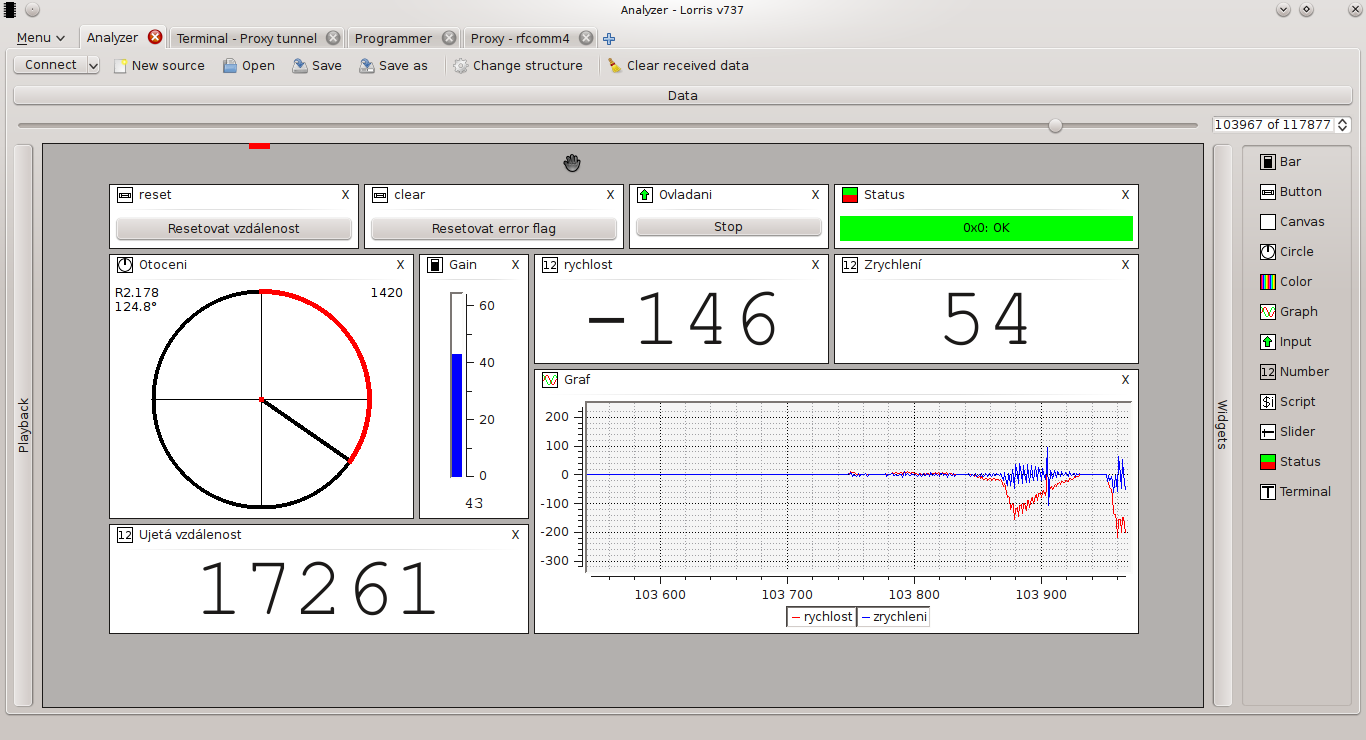
\includegraphics[width=\textwidth]{img/analyzer_all.png}
\caption{Modul analyzér}
\label{Analyzer}
\end{center}
\end{figure}

Tento modul parsuje data přicházející sériovou linkou a zobrazuje je v grafických "widgetech". Zpracovaná data je možné uložit a později zase v programu otevřít. Předpokládá se, že data mají formát packetů.

Struktura dat se nastavuje v samostatném dialogu (viz obrázek 3), kde je možno nastavit délku packetu, jeho endianess\cite{endian}, přitomnost hlavičky a její obsah -- statická data ("start byte"), délka packetu(pokud je proměnná), příkaz a ID zařízení. Podle příkazu a ID zařízení je možno později data filtrovat.

Po nastavení struktury se přijatá data začnou po packetech zobrazovat v horní části okna, a v pravé části se zobrazí sloupeček s dostupnými zobrazovacími widgety. Widgety se dají pomocí drag\&drop principu "vytahat" na plochu v prostřední části okna. Data se k widgetu přiřadí taktéž pomocí drag\&drop, tentokrát přetažení prvního bytu dat na widget. 

\newpage
\setlength{\voffset}{0mm} % posune text/obrázek na této stránce, kam patøí
\pagestyle{plain}

Poté widget zobrazuje data tohoto bytu, nebo tento byte bere jako první, pokud jsou data delší. Aby bylo možné zpětně poznat který byte je k widgetu přiřazen, je po najetí myši na widget červeně zvýrazněn.

Nastavení widgetu (jeho jméno, u čísla např. jeho datový typ apod.) jsou přistupná v kontextovém menu po pravém kliknutí myší na widget. Widgety je taktéž možné "uzamknout", aby nebylo možné je zavřít, měnit jejich pozici a velikost.

Aplikace si také přijatá data ukládá -- navigace je umožněna posuvníkem a boxem v horní části okna.

\subsection*{Widget: číslo}
\addcontentsline{toc}{subsection}{Widget: číslo}
\begin{figure}[h]
\begin{center}
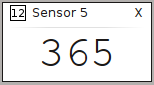
\includegraphics{img/w_num.png}
\end{center}
\end{figure}
Dokáže zobrazovat celá čísla (se znaménkem i bez, 8 až 64 bitů dlouhé) a desetiná čisla (single-precision\cite{float}, 32bit a 64bit -- jako v jazyku C).\\
Widget dokáže zarovnat číslo na maximální délku jeho datového typu\\a~formátovat ho těmito způsoby:
\begin{itemize}
    \item Desítkový -- číslo v desítkové soustavě
    \item Desítkový s exponentem -- použije exponent pro zapsaní velkých čísel. Dostupné pouze pro desetiná čísla.
    \item Hexadecimální -- výpis v šestnáctkové soustavě. Dostupné pouze pro typy bez znaménka. 
    \item Binární -- zobrazí číslo ve dvojkové soustavě
\end{itemize}

\newpage
\addcontentsline{toc}{subsection}{Widget: sloupcový bar}
\subsection*{Widget: sloupcový bar}
\begin{figure}[h]
\begin{center}
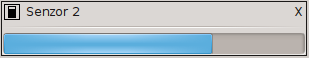
\includegraphics{img/w_bar.png}
\end{center}
\end{figure}
Zobrazuje hodnotu ve sloupcovém baru. Lze nastavit datový typ vstupních dat, orientaci (vertikální nebo horizontální) a rozmezí hodnot.

\addcontentsline{toc}{subsection}{Widget: barva}
\subsection*{Widget: barva}
\begin{figure}[h]
\begin{center}
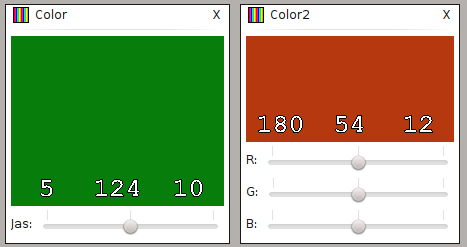
\includegraphics{img/w_col.png}
\end{center}
\end{figure}
Ukáže 24-bitové hodnoty RGB jako barevný obdélník. Dokáže provést korekci jasu a hodnot každé z barev RGB.

\newpage
\addcontentsline{toc}{subsection}{Widget: graf}
\subsection*{Widget: graf}
\begin{figure}[h]
\begin{center}
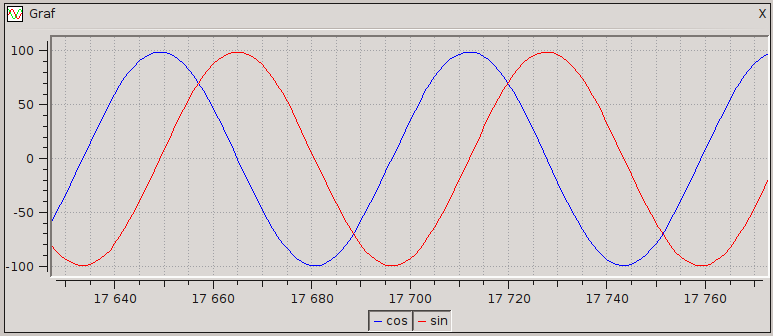
\includegraphics[scale=0.65]{img/w_graph.png}
\end{center}
\end{figure}
Zobrazuje hodnoty v grafu - osa Y jsou hodnoty, na ose X je počet vzorků. Lze nastavovat jméno, barvu a datový typ hrany, automatické posouvání grafu, velikost vzorku, měřítko os grafu a zobrazení legendy. Kliknutí na hranu v legendě grafu hranu skryje.
\begin{figure}[h]
\begin{center}
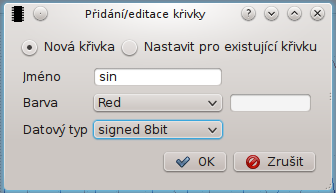
\includegraphics[scale=0.8]{img/w_graph_add.png}
\caption{Dialog pro nastavení parametrů hrany}
\end{center}
\end{figure}

% DOP: přímo ovládání grafu?


\newpage
\begin{figure}[h]
\begin{center}
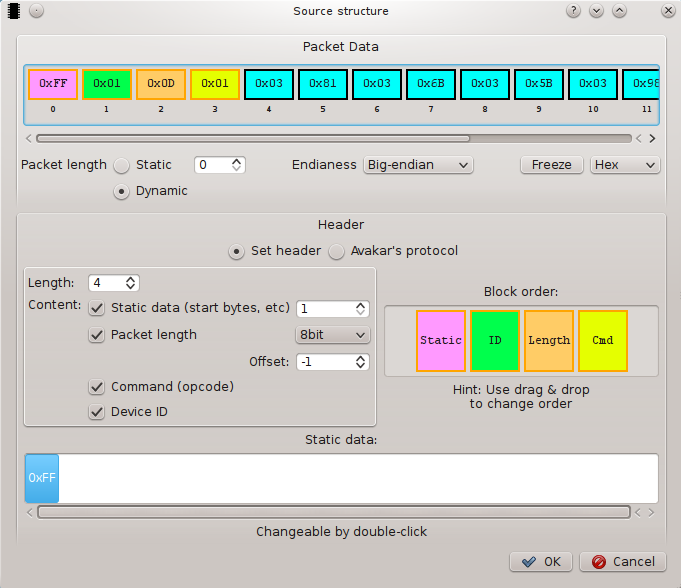
\includegraphics[scale=0.7]{img/analyzer_struct.png}
\caption{Dialog nastavení struktury dat}
\label{Analyzer_struct}
\end{center}
\end{figure}

\newpage
\setlength{\voffset}{0mm} % posune text/obrázek na této stránce, kam patøí
\pagestyle{plain}

\begin{figure}[H]
\begin{center}
\subfloat[Seznam widgetů]{\label{analyzer_widgets}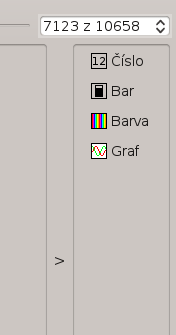
\includegraphics[scale=1]{img/analyzer_widgets.png}}
\hfill
\subfloat[Přiřazení dat pomocí drag\&drop]{\label{analyzer_widgets}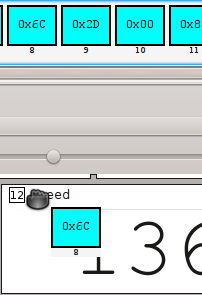
\includegraphics[scale=1]{img/analyzer_drag_data.png}}  
\caption{Widgety}
\label{widgets}
\end{center}
\end{figure}





\subsection*{Knihovny třetích stran}
{\bf Qwt}\cite{qwt_link} je knihovna pro Qt Framework obsahující tzv. widgety pro aplikace technického charakteru -- grafy, sloucové ukazatele, kompasy a podobně. Ve svojí práci
zatím z této knihovny používám pouze graf (v modulu analyzéru), ale v budoucnu bych chtěl použít i některé další součásti. \\
{\bf QExtSerialPort}\cite{qext_link} poskytuje připojení k sériovému portu a také dokáže vypsat seznam nalezených portů v počítačí.\\
{\bf QHexEdit2}\cite{qhex_link} je hex editor použitý v modulu programátoru Shupito na zobrazování obsahu paměti. V této knihovně jsem upravoval několik málo drobností, 
týkajících se především vzhledu.

\newpage
\setlength{\voffset}{0mm} % posune text/obrázek na této stránce, kam patøí
\pagestyle{plain}

\section*{Moduly}
\addcontentsline{toc}{section}{Moduly}
Každý modul se otevírá v samostatné záložce, přičemž je možné mít otevřeno více stejných modulů zároveň, a aby více modulů sdílelo jedno připojení (např. Teminál a Analyzér, oba pracující s jedním sériovým portem).
\subsection*{Současné moduly}
    \begin{itemize}
        \item Analyzér -- zobrazování dat v grafických widgetech, hlavní část práce.
        \item Proxy mezi Sériovým portem a TCP socketem -- umožňuje vzdálený přístup k sériovému portu
        \item Shupito -- rozhraní pro obsluhu programátoru "Shupito"\cite{shupito}
        \item Terminál -- terminál pro sériový port s podporou bootloaderu pro čipy ATmega\cite{avr232client}.
    \end{itemize}
\begin{figure}[h]
\begin{center}
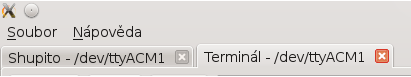
\includegraphics{img/tabs.png}
\caption{Záložky modulů}
\label{Moduly}
\end{center}
\end{figure}



\newpage
\setlength{\voffset}{0mm} % posune text/obrázek na této stránce, kam patøí
\pagestyle{plain}

\subsection*{Proxy mezi sériovým portem a TCP socketem}
\addcontentsline{toc}{subsection}{Proxy mezi sériovým portem a TCP socketem} 

\begin{figure}[h]
\begin{center}
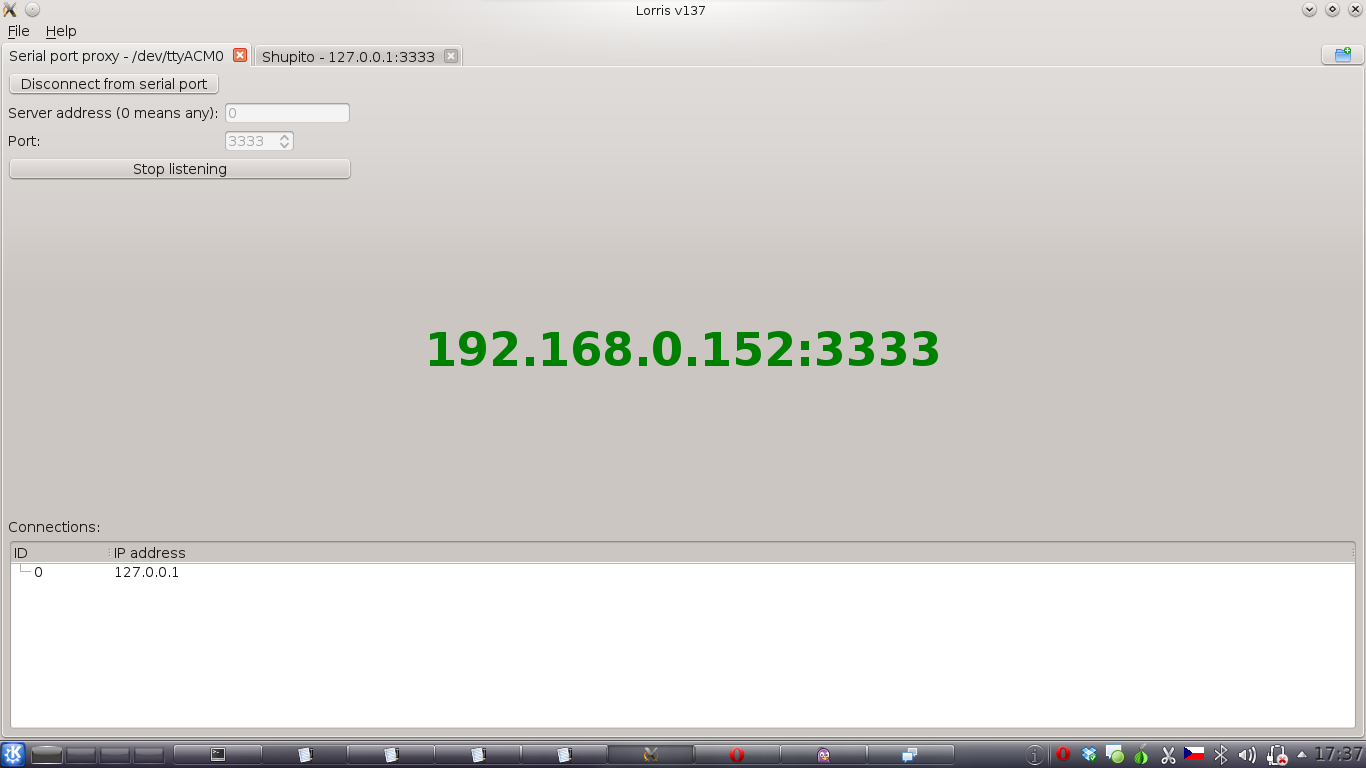
\includegraphics[width=\textwidth]{img/proxy.png}
\caption{Proxy mezi sériovým portem a TCP socketem}
\label{Shupito}
\end{center}
\end{figure}
Jednoduchá proxy mezi sériovým portem a TCP socketem, která umožňuje vzdálené připojení na sériový port, buďto z Lorris nebo jiného programu.


\newpage
\setlength{\voffset}{0mm} % posune text/obrázek na této stránce, kam patøí
\pagestyle{plain}

\subsection*{Shupito}
\addcontentsline{toc}{subsection}{Shupito} 

\begin{figure}[h]
\begin{center}
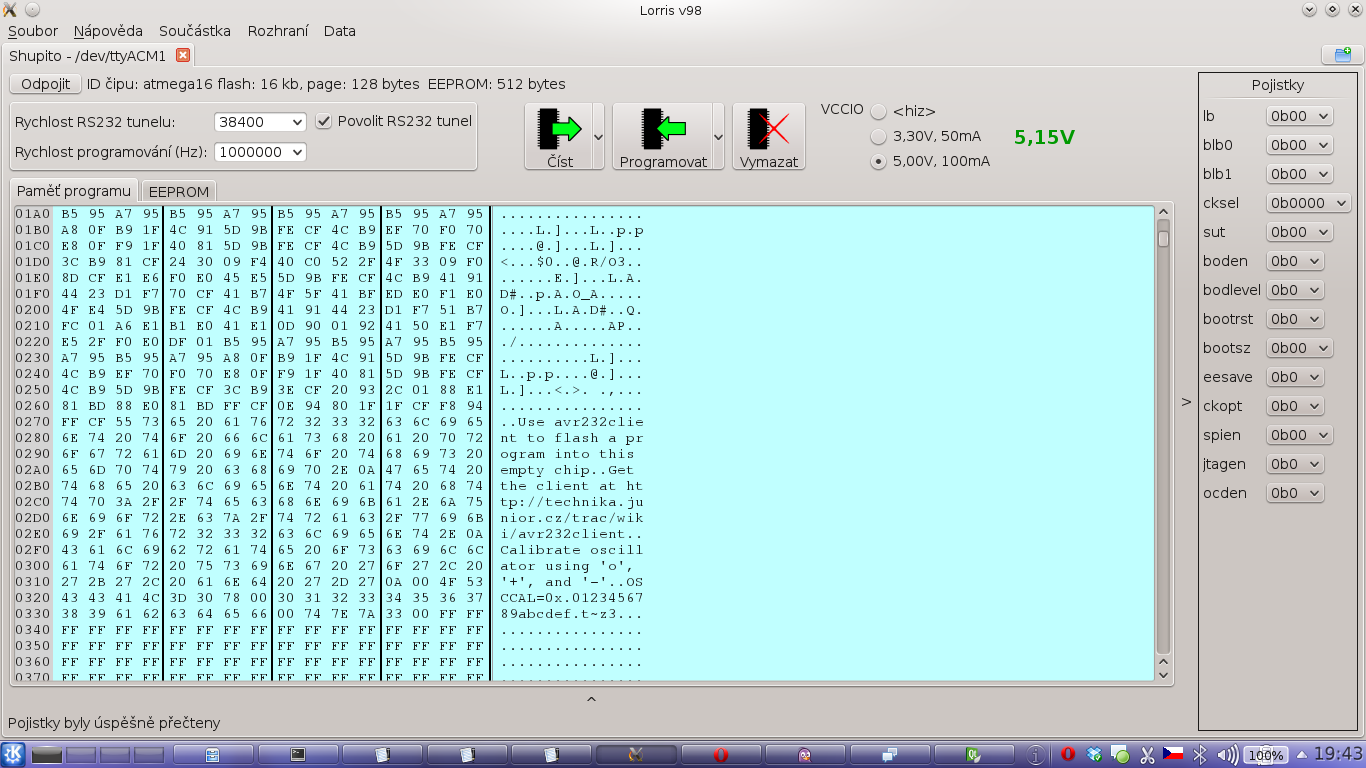
\includegraphics[width=\textwidth]{img/shupito.png}
\caption{Modul Shupito}
\label{Shupito}
\end{center}
\end{figure}
Shupito je programátor mikročipů vytvořený Martinem Vejnarem. Dokáže programovat mikrokontroléry pomocí ISP, PDI *DOP: zeptat se martina co všechno to zvládá*. 

Modul v mojí práci dokáže programátor Shupito obsluhovat -- nastavovat výstupní napětí, číst a programovat paměť čipů (flash i EEPROM) a číst a měnit pojistky. Jako výstupní i vstupní data používá soubory ve formátu Intel HEX32\cite{hex}. Shupito dokáže pracovat také jako RS232 tunel, i tuto funkci program podporuje -- aktivní tunel se zobrazí jako další typ připojení a je možné ho využívat v ostatních modulech.
Komunikace s programátorem je naportována z oficiálního ovládacího programu\cite{avr232client}, který je však dostupný pouze pro MS Windows.
\newpage
\setlength{\voffset}{0mm} % posune text/obrázek na této stránce, kam patøí
\pagestyle{plain}

\subsection*{Terminál}
\addcontentsline{toc}{subsection}{Terminál} 

\begin{figure}[h]
\begin{center}
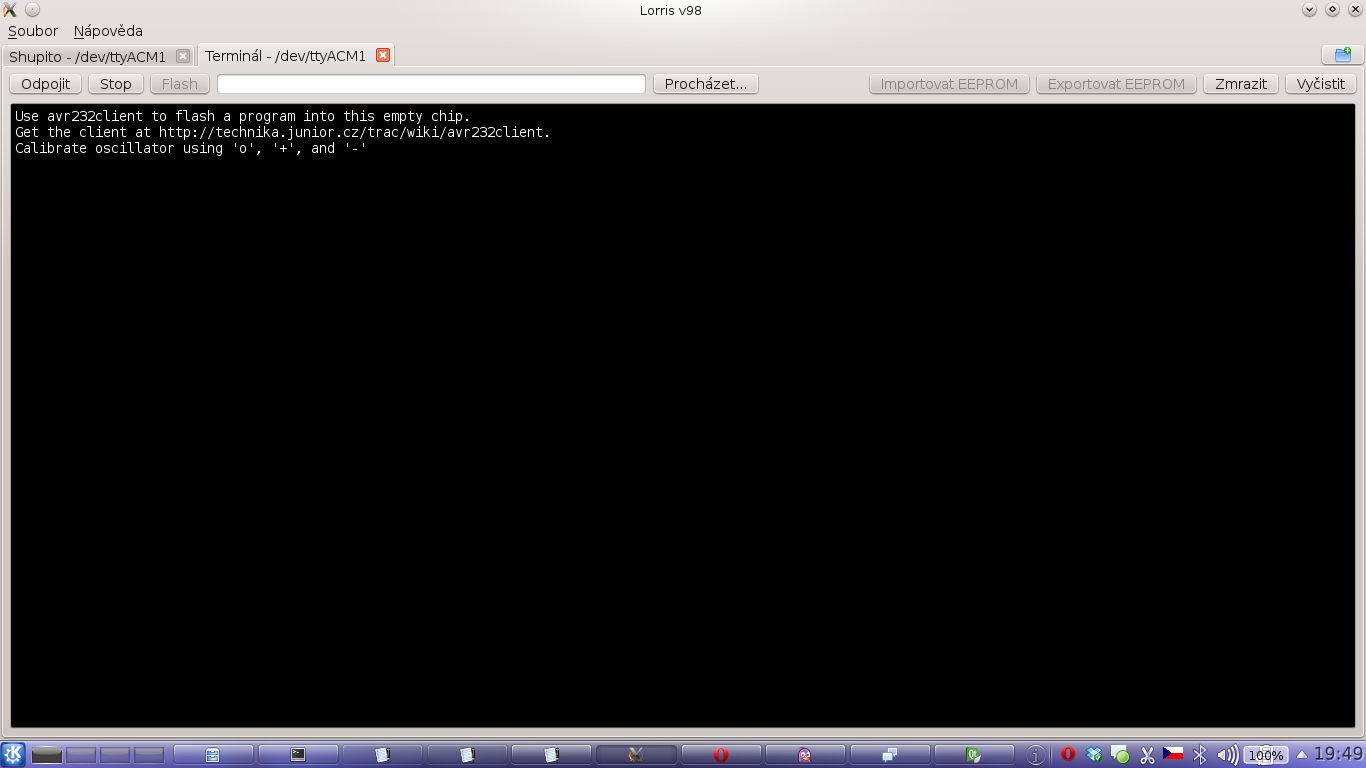
\includegraphics[width=\textwidth]{img/terminal.png}
\caption{Modul terminál}
\label{Terminal}
\end{center}
\end{figure}

Klasický terminál -- zobrazuje data přijatá přes sériový port a posílá stisky kláves, obohacený o podporu bootloaderu pro mikrokontroléry AVR ATmega(bootloader byl taktéž napsaný Martinem Vejnarem), který umožňuje jejich programování přes RS232 linku. Informace o protokolu bootloaderu jsem získal z oficiálního programu určeného k programování přes tento bootlodaer, avr232client\cite{avr232client}.

\newpage
\setlength{\voffset}{0mm} % posune text/obrázek na této stránce, kam patøí
\pagestyle{plain}

\section*{Možnosti dalšího rozšiřování programu}
\addcontentsline{toc}{section}{Možnosti dalšího rozšiřování programu}
Díky modulárnosti programu je možné poměrně jednoduše vytvořit \\ 
další moduly, například modul pro ovládání robota přes bluetooth pomocí joysticku apod. Je také možné přidat další typy připojení -- například socket, pokud jsou data nejdříve zpracována nějákým jiným programem.

Co se týče Analyzéru, je možné přidat další widgety -- mám v plánu implementaci QtScriptu\cite{qtscript}, který podstatně rozšíří možnosti parsování dat.

%%%%%%%%%%%%%%%%%%%%%%%%%%%%%%%%%%%%%%%%%%%%%%%%%%%%%%%%%%%%%%%%%%%%%%%%%%%
\newpage
\addcontentsline{toc}{section}{Reference}
 \begin{thebibliography}{99}
 %% 99 znamená, že maximální délka čísla literatury jsou dva znaky
% seznam samozřejmě změníte podle svého, tohle je pouze ukázka formátování
    \bibitem{qtfw} \It{Qt Framework -- Cross-platform application and UI framework} \\
    \url{http://qt.nokia.com/} (Stav ke dni 28.1.2012)

    \bibitem{tcp_sock} \It{TCP socket} \\
    \url{http://en.wikipedia.org/wiki/Transmission_Control_Protocol} (Stav ke dni 25.2.2012)

    \bibitem{repo} \It{GIT repozitář Lorris} \\
    \url{https://github.com/Tasssadar/Lorris}

    \bibitem{qwt_link} \It{Qt Widgets for Technical Applications} \\
    \url{http://qwt.sourceforge.net/} (Stav ke dni 22.2.2012)

    \bibitem{qext_link} \It{Qt interface class for old fashioned serial ports} \\
    \url{http://code.google.com/p/qextserialport/} \\
    (Stav ke dni 22.2.2012)

    \bibitem{qhex_link} \It{Binary Editor for Qt} \\
    \url{http://code.google.com/p/qhexedit2/} (Stav ke dni 22.2.2012)
    
    \bibitem{shupito} \It{Shupito -- Programátor} \\
    \url{http://shupito.net/} (Stav ke dni 28.1.2012)

    \bibitem{avr232client} \It{avr232client} \\
    \url{http://technika.junior.cz/trac/wiki/avr232client}\\
    (Stav ke dni 28.1.2012)

    \bibitem{endian} \It{Endianness} \\
    \url{http://en.wikipedia.org/wiki/Endianness} (Stav ke dni 28.1.2012)

    \bibitem{float} \It{Single-precision floating-point format} \\
    \url{http://en.wikipedia.org/wiki/Single_precision} (Stav ke dni 28.1.2012)

    \bibitem{hex} \It{Intel HEX} \\
    \url{http://en.wikipedia.org/wiki/Intel_hex} (Stav ke dni 28.1.2012)
    
    \bibitem{qtscript} \It{QtScript} \\
    \url{http://developer.qt.nokia.com/doc/qt-4.7/qtscript.html} (Stav ke dni 28.1.2012)    
\end{thebibliography}

\end{document}